\chapter{Einleitung}

\begin{itemize}
    \item Schüttgutsortierung ist ein wichtiges Thema \todo{hier vielleicht dieses 10\% der Energie Beispiel bringen?}
    \item Anwendungsbereiche Schüttgutsortierung
    \item Maschinelle Lernverfahren sind ein heißes Thema, dass bei vielen existierenden problemen Anwendung findet
\end{itemize}

\todo{Einleitungstext}

\section{Motivation}

\color{blue}
\begin{itemize}
    \item State of the Art: große Sortierer 
    \item Kooperation ISAS IOSB, \textit{TrackSort} Projekt 
    \item Flächenkamera
    \item 2 geteiltes Problem: Tracking und Prediction
    \item Fokus dieser Arbeit: Prediction
    \item Bewegungsmodelle für verschiedene Schüttgüter von Hand finetunen ist viel Aufwand und schwer
    \item Option: Neuronale Netze einsetzen! 
    \item zwei verschiedene Problemstellungen:
    \item 1. die Position des Teilchens im nächsten Zeitschritt. \textbf{NextStep} für Trackingphase
    \item 2. die Position (und die Zeit) die das Teilchen beim Passieren des Düsenarrays haben wird. \textbf{Separator}
    \item Aktuell: auf Messungen - kein Vollständiger Schätzer
\end{itemize}
\color{black}

\todo[inline]{arbeit motivieren. Schüttgutsortierung ist ein interessantes Feld, das sich potenziell für ML anbietet.}
\todo[inline]{auf jeden fall separator und nextStep Netze unterscheidung erwähnen}


Im Rahmen dieser Arbeit sollen zwei verschiedene Prädiktionsprobleme mittels neuronaler Netze gelöst werden.
Einerseits soll vorhergesagt werden, an welcher Position sich ein Teilchen im nächsten Zeitschritt befinden wird.
Diese Netze werden im Rahmen dieser Netze als NextStep Netze bezeichnet.
Eine Visualisierung dieser Aufgabe ist in Abbildung~\ref{fig:visualsNextstep} zu sehen.
Andererseits soll vorhergesagt werden an welcher Position und wann ein Teilchen das Druckluftdüsenarray passieren wird.
Diese Problemstellung wird von den sogenannten Separator Netzen gelöst.
Eine Visualisierung dieser Aufgabe ist in Abbildung~\ref{fig:visualsSeparator} zu sehen.

\todo[inline]{Visualisierung von Separator Netz output}

\begin{figure}[h]
    \centering
    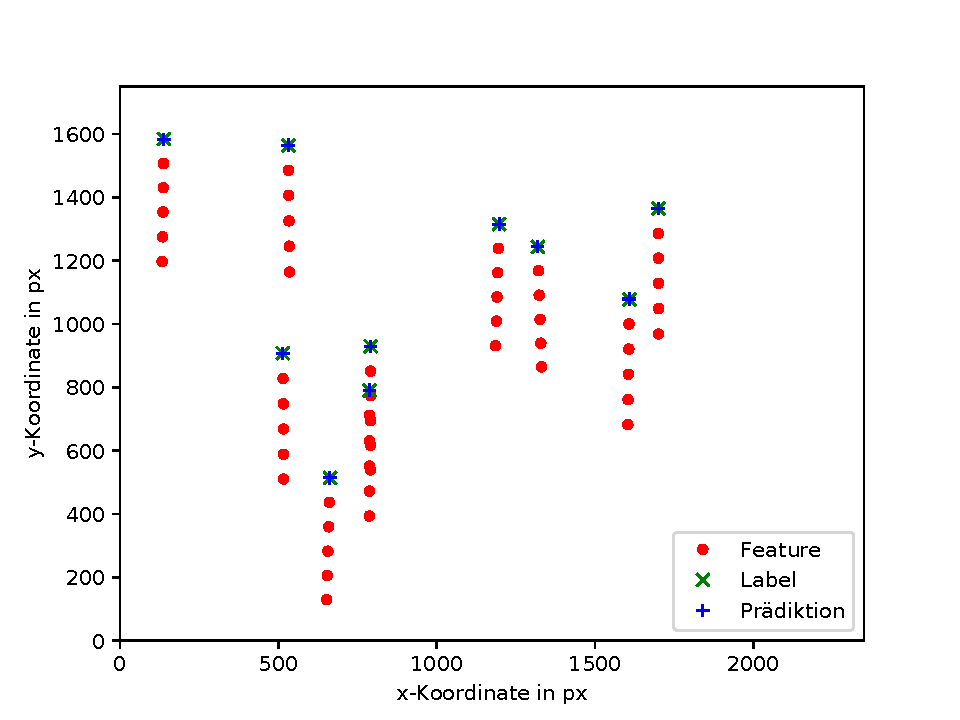
\includegraphics[width=\textwidth]{NextStep-45kDecaySteps-ZylinderReal_2018-11-29.pdf}
    \caption{Visualisierung einer gelösten Probleminstanz eines NextStep Netzes}
    \label{fig:visualsNextstep}
\end{figure}


\begin{figure}[h]
    \centering
    \missingfigure{Boxplots Result NeuralNets NextStep}
	% 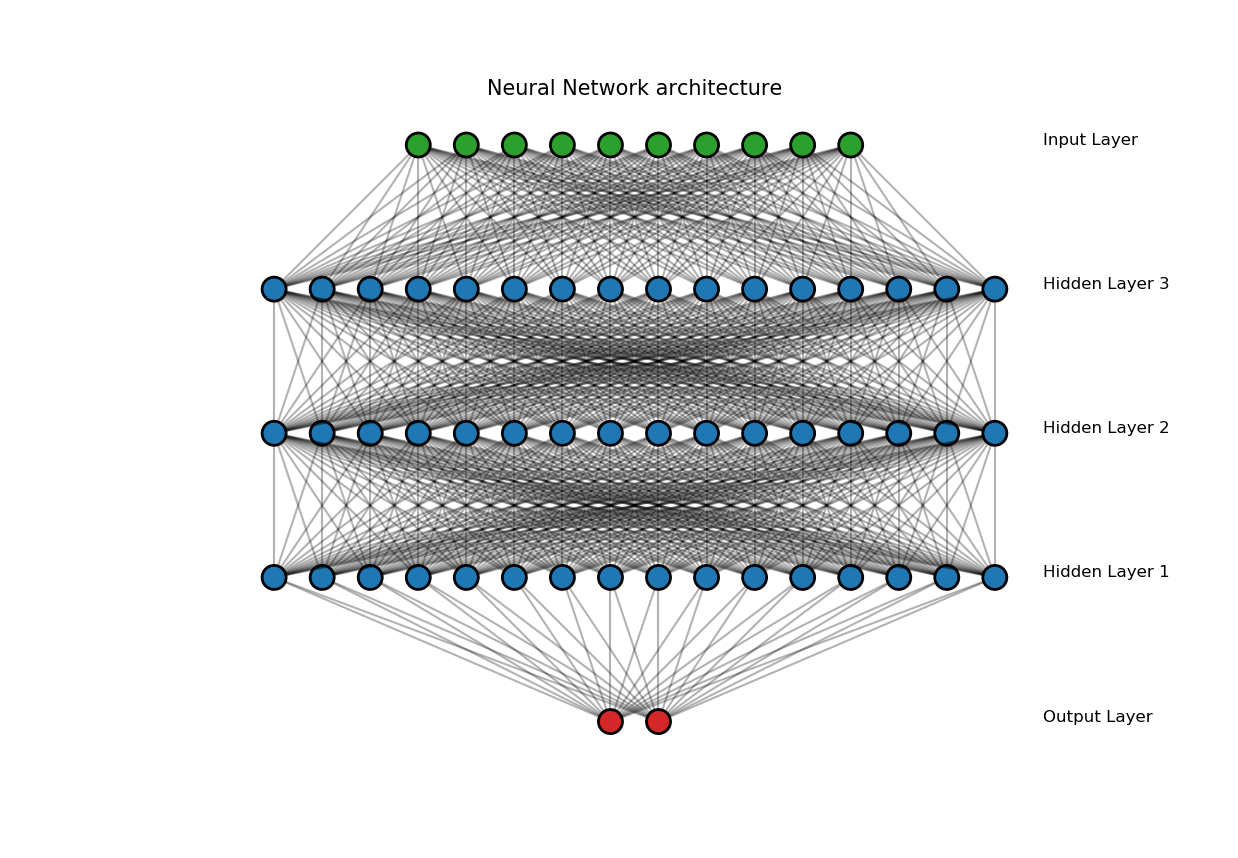
\includegraphics[width=\textwidth]{NN_NextStep_v2}
	\caption{Visualisierung einer gelösten Probleminstanz eines Separator Netzes}
	% \todo{Quelle Bild!}
	\label{fig:visualsSeparator}
\end{figure}



\section{Aufbau der Arbeit}

Das schreibe ich auf, wenn die Gliederung finalisiert ist.

\todo{aufbau Gliederung beschreiben. Ganz am Ende dann, wenn sich nichts mehr ändert}

